\documentclass[12pt,a4paper]{article}
\usepackage[utf8]{inputenc}
\usepackage{amsmath}
\usepackage{amsfonts}
\usepackage{amssymb}
\usepackage{graphicx}
\usepackage{tikz}
\usepackage{pgfplots}
\usepackage{listings}
\usepackage{xcolor}
\usepackage{geometry}
\usepackage{hyperref}
\usepackage{float}
\usepackage{subcaption}
\usetikzlibrary{positioning}

\geometry{margin=1in}

% Code listing style
\lstset{
    language=C,
    basicstyle=\ttfamily\small,
    keywordstyle=\color{blue},
    commentstyle=\color{green!60!black},
    stringstyle=\color{red},
    numbers=left,
    numberstyle=\tiny,
    frame=single,
    breaklines=true,
    showstringspaces=false
}

% Update title
\title{CSE-406 Project : DNS Cache Poisoning and Phishing Attack}
\author{
    Kowshik Saha\\
    ID: 2005006
    \and
    Fairuz Mubashwera\\
    ID: 2005030
}

\date{\today}

\begin{document}

\maketitle

\tableofcontents
\newpage

\section{Introduction}

This report presents a design proposal of a two-stage network attack: DNS Cache Poisoning followed by a phishing attack. The first stage corrupts the DNS resolver's cache, redirecting traffic for a target domain to an attacker-controlled IP. The second stage leverages this redirection to present a phishing site, harvesting user credentials. This end-to-end attack demonstrates the real-world impact of DNS vulnerabilities.

\section{Definition of the Attack}

\subsection{Attack Overview}

The attack consists of two phases:
\begin{enumerate}
    \item \textbf{DNS Cache Poisoning}: DNS cache poisoning is a cyberattack in which a malicious actor injects forged DNS responses into the cache of a DNS resolver. The goal is to corrupt the resolver's memory by making it associate a domain name with a fake IP address controlled by the attacker.
    
In a typical DNS lookup, a resolver queries authoritative servers to resolve domain names into IP addresses. If the attacker can successfully send a spoofed DNS response before the legitimate one arrives — with the correct transaction ID, source port, and spoofed source IP — the resolver will accept and cache the malicious response \cite{rfc1035}.

Once poisoned, the resolver will serve the attacker’s IP for all future queries to the targeted domain. This allows the attacker to redirect users to phishing sites without the knowledge of victim.

    \item \textbf{Phishing}: Phishing is a form of cyberattack in which an attacker impersonates a legitimate entity to deceive users into revealing sensitive information such as usernames, passwords, or financial details. This is often carried out through fake websites or emails that closely mimic trusted sources. The goal is to exploit the user’s trust and familiarity with these entities in order to harvest confidential data or deliver malware. 

One method attackers use to carry out phishing more convincingly is DNS cache poisoning. By corrupting the cache of a DNS resolver, the attacker can redirect traffic for a legitimate domain to a malicious server without altering the domain name shown in the user's browser . Because the URL appears correct and the page looks authentic, users are more likely to enter their credentials or other sensitive data, unknowingly handing them over to the attacker. 
\end{enumerate}

\subsection{Kaminsky Attack Variant of DNS Cache Poisoning}

The proposed design uses the Kaminsky attack technique, which exploits the birthday paradox to significantly increase the success probability of cache poisoning. Instead of targeting a single transaction, the attack\cite{rfc4033}:

\begin{enumerate}
    \item Sends multiple parallel DNS queries for random subdomains
    \item Floods the target resolver with spoofed responses
    \item Exploits the birthday paradox to match transaction IDs
    \item Poisons the authority section with malicious nameserver information
\end{enumerate}

\subsection{Attack Objectives}

The primary objectives of this DNS cache poisoning attack are:

\begin{itemize}
    \item \textbf{Cache Corruption}: Inject false DNS records into the target resolver's cache
    \item \textbf{Traffic Redirection}: Redirect legitimate traffic to attacker-controlled servers
    \item \textbf{Authority Poisoning}: Replace legitimate nameservers with malicious ones
    \item \textbf{Persistence}: Maintain the poisoned state for extended periods
\end{itemize}



\section{Topology Diagram}

% Topology Diagram
\begin{figure}[H]
\centering
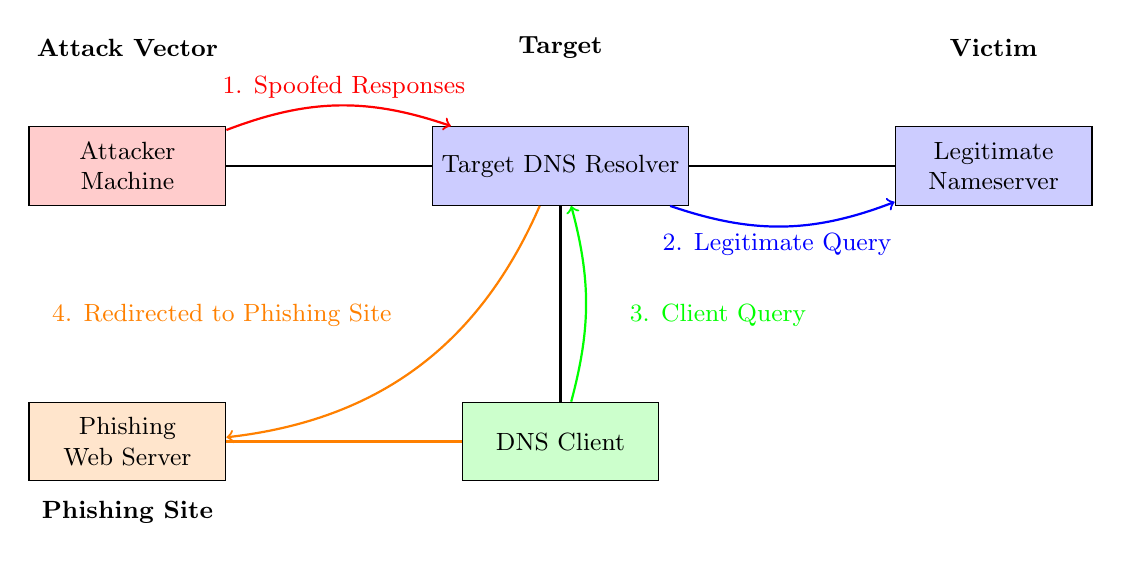
\begin{tikzpicture}[
    every node/.style={font=\small},
    box/.style={rectangle,draw,minimum width=2.5cm,minimum height=1cm,align=center},
    attack/.style={box,fill=red!20},
    server/.style={box,fill=blue!20},
    client/.style={box,fill=green!20},
    phishing/.style={box,fill=orange!20}
]

% Node grid moved down
\node[attack]   (attacker)   at (0,-0.8)     {Attacker\\Machine};
\node[server]   (resolver)   at (5.5,-0.8)   {Target DNS Resolver};
\node[server]   (legit_ns)   at (11,-0.8)    {Legitimate\\Nameserver};
\node[phishing] (phish)      at (0,-4.3)       {Phishing\\Web Server};
\node[client]   (client)     at (5.5,-4.3)     {DNS Client};

% Labels above top row
\node[align=center] at (0,0.7)     {\textbf{Attack Vector}};
\node[align=center] at (5.5,0.7)   {\textbf{Target}};
\node[align=center] at (11,0.7)    {\textbf{Victim}};
% Label below phishing site
\node[align=center] at (0,-5.2)    {\textbf{Phishing Site}};

% Network connections (basic lines)
\draw[thick] (attacker) -- (resolver);
\draw[thick] (resolver) -- (legit_ns);
\draw[thick] (client) -- (resolver);
\draw[thick,orange] (client) -- (phish);

% Attack flow arrows with adjusted label positions
\draw[->,red,thick] (attacker) to[bend left=20] (resolver);
\node[red] at (2.75,0.2) {1. Spoofed Responses};

\draw[->,blue,thick] (resolver) to[bend right=20] (legit_ns);
\node[blue] at (8.25,-1.8) {2. Legitimate Query};

\draw[->,green,thick] (client) to[bend right=15] (resolver);
\node[green] at (7.5,-2.7) {3. Client Query};

\draw[->,orange,thick] (resolver) to[bend left=30] (phish);
\node[orange] at (1.2,-2.7) {4. Redirected to Phishing Site};

\end{tikzpicture}
\caption{Network Topology: DNS Cache Poisoning and Phishing}
\label{fig:topology}
\end{figure}


\subsection{Network Components}

\begin{description}
    \item[Attacker Machine] The system running the DNS cache poisoning tool, capable of generating spoofed DNS packets
    \item[Target DNS Resolver] The recursive DNS server whose cache is to be poisoned
    \item[Legitimate Nameserver] The authoritative DNS server for the target domain
    \item[DNS Client] Regular clients that query the poisoned resolver
\end{description}

\section{Timing Diagrams}

\subsection{Original DNS Protocol Timing}

\begin{figure}[H]
\centering
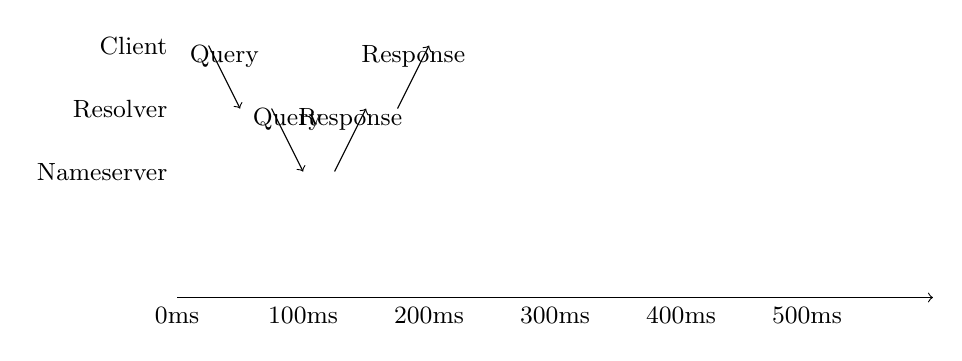
\begin{tikzpicture}[
    scale=0.8,
    every node/.style={font=\small}
]

% Timeline
\draw[->] (0,0) -- (12,0);
\node[below] at (0,0) {0ms};
\node[below] at (2,0) {100ms};
\node[below] at (4,0) {200ms};
\node[below] at (6,0) {300ms};
\node[below] at (8,0) {400ms};
\node[below] at (10,0) {500ms};

% Actors
\node[left] at (0,4) {Client};
\node[left] at (0,3) {Resolver};
\node[left] at (0,2) {Nameserver};

% Normal DNS flow
\draw[->] (0.5,4) -- (1,3) node[midway,above] {Query};
\draw[->] (1.5,3) -- (2,2) node[midway,above] {Query};
\draw[->] (2.5,2) -- (3,3) node[midway,above] {Response};
\draw[->] (3.5,3) -- (4,4) node[midway,above] {Response};

\end{tikzpicture}
\caption{Normal DNS Resolution Timing}
\label{fig:normal_timing}
\end{figure}

\subsection{Attack Timing Diagram}

\begin{figure}[H]
\centering
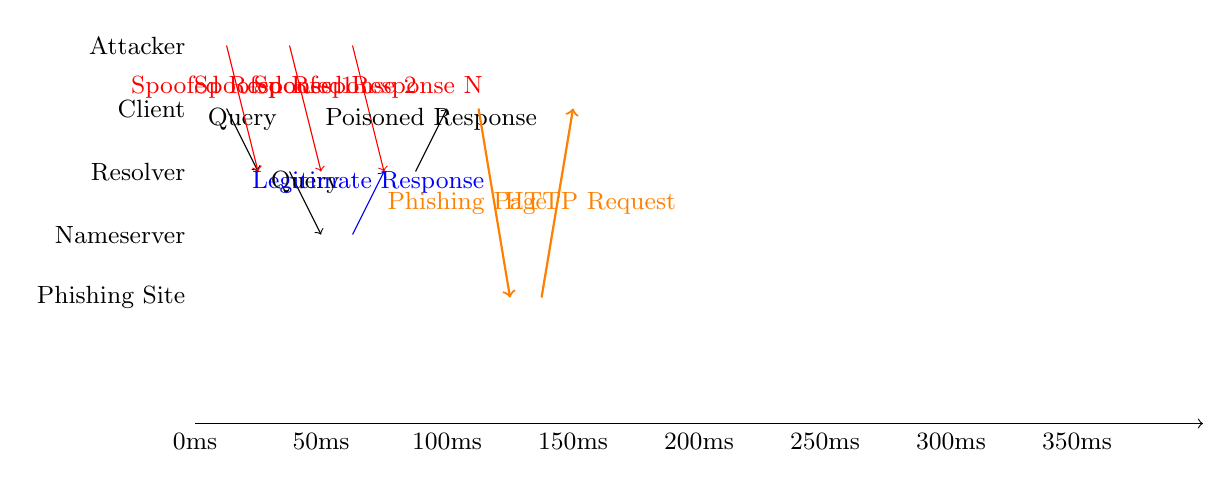
\begin{tikzpicture}[
    scale=0.8,
    every node/.style={font=\small}
]

% Timeline
\draw[->] (0,0) -- (16,0);
\node[below] at (0,0) {0ms};
\node[below] at (2,0) {50ms};
\node[below] at (4,0) {100ms};
\node[below] at (6,0) {150ms};
\node[below] at (8,0) {200ms};
\node[below] at (10,0) {250ms};
\node[below] at (12,0) {300ms};
\node[below] at (14,0) {350ms};

% Actors
\node[left] at (0,6) {Attacker};
\node[left] at (0,5) {Client};
\node[left] at (0,4) {Resolver};
\node[left] at (0,3) {Nameserver};
\node[left] at (0,2) {Phishing Site};

% Attack flow
\draw[->] (0.5,5) -- (1,4) node[midway,above] {Query};
\draw[->] (1.5,4) -- (2,3) node[midway,above] {Query};

% Parallel attack
\draw[->,red] (0.5,6) -- (1,4) node[midway,above,red] {Spoofed Response 1};
\draw[->,red] (1.5,6) -- (2,4) node[midway,above,red] {Spoofed Response 2};
\draw[->,red] (2.5,6) -- (3,4) node[midway,above,red] {Spoofed Response N};

% Race condition
\draw[->,blue] (2.5,3) -- (3,4) node[midway,above,blue] {Legitimate Response};

% Poisoned response
\draw[->] (3.5,4) -- (4,5) node[midway,above] {Poisoned Response};

% Phishing
\draw[->,orange,thick] (4.5,5) -- (5,2) node[midway,right,orange] {HTTP Request};
\draw[->,orange,thick] (5.5,2) -- (6,5) node[midway,left,orange] {Phishing Page};

\end{tikzpicture}
\caption{Attack Timing: DNS Poisoning and Phishing}
\label{fig:attack_timing}
\end{figure}

\subsection{Attack Strategy}

The attack employs a sophisticated timing strategy:

\begin{enumerate}
    \item \textbf{Parallel Query Generation}: Multiple DNS queries for random subdomains are sent simultaneously
    \item \textbf{Response Flooding}: A large number of spoofed responses are sent immediately after the queries
    \item \textbf{Race Condition Exploitation}: The attacker races against legitimate responses
    \item \textbf{Birthday Paradox Utilization}: Multiple queries increase the probability of transaction ID collision
\end{enumerate}

\section{Packet and Frame Details}

\subsection{DNS Query Packet Structure}

The DNS query packet is constructed with the following fields\cite{cert-dns}:

\begin{table}[H]
\centering
\begin{tabular}{|l|p{8cm}|}
\hline
\textbf{Field} & \textbf{Description} \\
\hline
Transaction ID & Random 16-bit identifier  used to match requests and responses. \\
\hline
Flags & Set to \texttt{DNS\_FLAG\_QUES}, indicating a DNS query packet. \\
\hline
Questions (QDCOUNT) &  the number of queries included. \\
\hline
Answer RRs (ANCOUNT) &  number of answers are present in the query. \\
\hline
Authority RRs & number of authority records included. \\
\hline
Additional RRs & number of  additional records included. \\
\hline
Question Section & Contains a single query record specifying: \\
& \quad - Query type . \\
& \quad - Query class . \\
& \quad - Query name . \\
\hline
\end{tabular}
\caption{Structure of the DNS query packet}
\end{table}

\vspace{1em}

\subsection{Spoofed DNS Response Packet Structure}

The spoofed DNS response packet includes the following fields\cite{cert-dns}:

\begin{table}[H]
\centering
\begin{tabular}{|l|p{8cm}|}
\hline
\textbf{Field} & \textbf{Description} \\
\hline
Transaction ID & Random 16-bit identifier, attempting to match the resolver’s expected transaction ID. \\
\hline
Flags & Set to \texttt{DNS\_FLAG\_RESP}, indicating a DNS response packet. \\
\hline
Questions (QDCOUNT) & same query as in the original request. \\
\hline
Answer RRs (ANCOUNT) & number of answer record. \\
\hline
Authority RRs & number of authority record. \\
\hline
Additional RRs & number of  additional record (glue record). \\
\hline
Question Section & Repeats the original query: \texttt{A} record for the random subdomain. \\
\hline
Answer Section & Provides a fake  record mapping the random subdomain to the attacker-controlled IP address. \\
\hline
Authority Section & Sets the nameserver (\texttt{NS}) record for the domain to an attacker-controlled nameserver. \\
\hline
Additional Section & Provides the record (IP address) of the attacker-controlled nameserver (glue record). \\
\hline
\end{tabular}
\caption{Structure of the spoofed DNS response packet}
\end{table}


\subsection{IP Header Modifications}

The design proposes raw IP packets with the following modifications:

\begin{table}[H]
\centering
\begin{tabular}{|l|l|l|}
\hline
\textbf{Field} & \textbf{Modified Value} & \textbf{Purpose} \\
\hline
Source IP & Original Nameserver IP & Spoofing \\
Destination IP & Target Resolver IP & Targeting \\
Protocol & UDP (17) & DNS Transport \\
TTL & 64 & Network traversal \\
\hline
\end{tabular}
\caption{IP Header Modifications}
\label{tab:ip_header}
\end{table}

\subsection{UDP Header Modifications}

\begin{table}[H]
\centering
\begin{tabular}{|l|l|l|}
\hline
\textbf{Field} & \textbf{Modified Value} & \textbf{Purpose} \\
\hline
Source Port & 53 (DNS) & Appear as DNS server \\
Destination Port & Resolver's port & Target specific port \\
Length & Calculated & Packet size \\
Checksum & Calculated & Valid packet \\
\hline
\end{tabular}
\caption{UDP Header Modifications}
\label{tab:udp_header}
\end{table}

\subsection{DNS Header Structure}

\begin{table}[H]
\centering
\begin{tabular}{|l|l|l|}
\hline
\textbf{Field} & \textbf{Size} & \textbf{Description} \\
\hline
Transaction ID & 16 bits & Random identifier \\
Flags & 16 bits & Response flags \\
Question Count & 16 bits & Number of questions \\
Answer Count & 16 bits & Number of answers \\
Authority Count & 16 bits & Number of authority records \\
Additional Count & 16 bits & Number of additional records \\
\hline
\end{tabular}
\caption{DNS Header Structure}
\label{tab:dns_header}
\end{table}

\subsection{Resource Record Structure}

The spoofed response includes multiple resource records:

\begin{enumerate}
    \item \textbf{Answer Record}: Maps random subdomain to attacker IP
    \item \textbf{Authority Record}: Declares attacker as nameserver for target domain
    \item \textbf{Additional Record}: Provides IP address for attacker nameserver
\end{enumerate}

\section{Phishing Attack Details}

\subsection{Phishing Site Setup}

After successful DNS cache poisoning, users attempting to visit the target domain are transparently redirected to a phishing site hosted by the attacker. This site mimics the legitimate website and is designed to capture sensitive credentials (e.g., usernames, passwords).

\subsection{Credential Harvesting Flow}

\begin{enumerate}
    \item User enters the target domain in their browser
    \item DNS resolver returns the attacker's IP (due to poisoning)
    \item User's browser connects to the phishing server
    \item Phishing site presents a fake login page
    \item User submits credentials, which are stored by the attacker
\end{enumerate}

\subsection{Phishing Page Example}

\begin{lstlisting}[language=HTML,caption=Example Phishing Login Page]
<!DOCTYPE html>
<html>
<head><title>Login</title></head>
<body>
<h2>Login to Your Account</h2>
<form method="POST" action="/steal">
  Username: <input type="text" name="user"><br>
  Password: <input type="password" name="pass"><br>
  <input type="submit" value="Login">
</form>
</body>
</html>
\end{lstlisting}

\subsection{Packet/Frame Details for Phishing}

After DNS poisoning, the following packets are observed:
\begin{itemize}
    \item HTTP GET/POST requests from client to phishing server
    \item HTTP responses containing fake login forms
    \item POST requests containing stolen credentials
\end{itemize}

\section{Design Justification}

\subsection{Why This Design Should Work}

\subsubsection{ Birthday Paradox Exploitation}

The attack leverages the birthday paradox \cite{feng-dns} to increase success probability:

\begin{equation}
P(\text{collision}) = 1 - \frac{365!}{(365-n)! \times 365^n}
\end{equation}

With K parallel requests and M spoofed responses, the probability of at least one transaction ID match is significantly higher than the naive 1/65536.

\subsubsection{ Race Condition Advantage}

The attack creates a race condition between:
\begin{itemize}
    \item Legitimate DNS responses from authoritative servers
    \item Spoofed responses from the attacker
\end{itemize}

By flooding the target with responses immediately after queries, the attacker increases the chance of winning the race.

\subsubsection{ Authority Section Poisoning}

The attack specifically targets the authority section, which contains nameserver information. This provides:

\begin{itemize}
    \item \textbf{Persistence}: Poisoned nameserver information remains in cache
    \item \textbf{Amplification}: Future queries for the domain will be directed to attacker
    \item \textbf{Scope}: Affects all subdomains of the target domain
\end{itemize}

\subsubsection{ Random Subdomain Strategy}

Using random subdomains provides several advantages:

\begin{itemize}
    \item \textbf{Cache Miss Guarantee}: Random subdomains are unlikely to be cached
    \item \textbf{Query Generation}: Forces the resolver to query authoritative servers
    \item \textbf{Attack Window}: Creates predictable timing for response injection
\end{itemize}

\subsection{End-to-End Attack Justification}

Combining DNS cache poisoning with phishing maximizes the attack's impact:
\begin{itemize}
    \item \textbf{Stealth}: Users are unaware of redirection
    \item \textbf{Effectiveness}: High likelihood of credential theft
    \item \textbf{Persistence}: Poisoned cache can affect many users
    \item \textbf{Scalability}: Attack can target any domain
\end{itemize}




\section{Conclusion}

This report proposes a design for a full attack chain: DNS cache poisoning followed by phishing. By corrupting the resolver's cache, the attacker transparently redirects users to a phishing site, enabling large-scale credential theft. 

The design's effectiveness is justified through:
\begin{itemize}
    \item Mathematical exploitation of the birthday paradox
    \item Strategic timing and race condition manipulation
    \item Comprehensive packet crafting and spoofing
\end{itemize}


\begin{thebibliography}{9}

\bibitem{feng-dns}
Wuchang Feng, \textit{CS510 Network Security Lecture Notes}, Fall 2005.  
Available at: \url{https://www.thefengs.com/wuchang/courses/old_courses/cs510netsec_fall2005/summaries/10.pdf}

\bibitem{rfc1035}
P. Mockapetris, \textit{RFC 1035: Domain Names - Implementation and Specification}, November 1987.  
Available at: \url{https://datatracker.ietf.org/doc/html/rfc1035}

\bibitem{rfc4033}
R. Arends et al., \textit{RFC 4033: DNS Security Introduction and Requirements}, March 2005.  
Available at: \url{https://datatracker.ietf.org/doc/html/rfc4033}

\bibitem{cert-dns}
CERT Coordination Center, \textit{DNS Cache Poisoning – The Next Generation}, April 2008.  
Available at: \url{https://www.kb.cert.org/vuls/id/800113}

\end{thebibliography}


\end{document} 
